\documentclass[aspectratio=169,12pt]{beamer}
\usetheme{Madrid}
\usecolortheme{dolphin}
\usefonttheme{professionalfonts}
\setbeamertemplate{navigation symbols}{}
\setbeamertemplate{footline}{}

\usepackage[T1]{fontenc}
\usepackage[utf8]{inputenc}
\usepackage{graphicx}
\usepackage{amsmath,amssymb}
\usepackage{hyperref}
\usepackage{siunitx}
\usepackage{physics}

\title[Chapitre 1]{Chapitre 1: Démystification}
\author{JAMOTTE Maxime, SCHOONEN Cédric}
\institute{Digital Learning Hub}
\date{}

\begin{document}

\begin{frame}
  \titlepage
\end{frame}

\begin{frame}{Plan}
  \begin{enumerate}
    \item Notre Univers est quantique: 4 phénomènes clefs.
    \\~\\
    \item Différences fondamentales entre ordinateurs classique et quantique.
    \\~\\
    \item Pourquoi recourir aux ordinateurs (et simulateurs) quantiques ?
  \end{enumerate}
\end{frame}

\section{Notre Univers est quantique}

\begin{frame}{Quatre phénomènes clefs}
  \begin{itemize}
    \item Stabilité de l'atome.
    \item Raies spectrales.
    \item Diffraction d'électrons (fentes de Young).
    \item Expérience de Stern-Gerlach.
  \end{itemize}
\end{frame}

\begin{frame}{Stabilité de l'atome}
  \begin{itemize}[<+->]
    \item Un charge qui tourne émet des ondes, donc \textbf{perd} de l'énergie. Donc l'électron devrait spiraler et s'effondrer sur le noyau.
    \begin{figure}
      \includegraphics[width=0.2\linewidth]{figures/class_electron.png}
    \end{figure}
    \item Or la matière ne s'effondre pas, elle est stable.\\~\\
    \item Mécanique quantique: niveau d'énergie minimale stable + niveaux d'énergie quantifiés: modèle de Bohr (1910s).\\~\\
    \item Les transitions se font par paquets d'énergie précis (photons).
  \end{itemize}
\end{frame}

\begin{frame}{Raies spectrales}
  \begin{itemize}[<+->]
    \item Spectre d'émission du soleil (Fraunhofer, 1814).
    \begin{figure}
      \includegraphics[width=0.6\linewidth]{figures/Fraunhofer_lines.png}
    \end{figure}
    \item Raies sombres dues à l'absorption des gaz dans le soleil et de notre atmosphère (Bunsen et Kirchhoff, 1859).
    \\~\\
    \item Les raies spectrales signent ces sauts discrets entre orbitales (Bohr).
  \end{itemize}
\end{frame}

\begin{frame}{Diffraction d'électrons (1927)}
  \begin{itemize}
    \item Les électrons passent par deux fentes. Classiquement, on s'attend à deux bandes.
  \end{itemize}
\end{frame}

\begin{frame}{Diffraction d'électrons (1927)}
  \begin{itemize}[<+->]
    \item Les électrons passent par deux fentes. Classiquement, on s'attend à deux bandes.
    \begin{figure}
      \includegraphics[width=0.3\linewidth]{figures/fente_Young.pdf}
    \end{figure}
    \item Même envoyés un par un, le motif d'interférence apparaît -- comme pour les ondes lumineuses (Young, 1801).
    \item La mécanique classique ne peut expliquer ce double comportement onde-particule.
    \item Chaque électron \textbf{interfère avec lui-même} car il passe par les deux fentes 
    \textbf{en même temps}. Il est à deux endroits en même temps, donc on ne sait pas où exactement.
  \end{itemize}
  \vfill
  \hfill\href{https://www.youtube.com/watch?v=JlsPC2BW_UI&list=PL_wN0FeVwhX6yH4bIQdHEvuPAQqWJM84M}{Vidéo fentes de Young}
\end{frame}

\begin{frame}{Expérience de Stern-Gerlach (1922)}
  \begin{itemize}[<+->]
    \item Faisceau d'atomes d'argent dans un champ magnétique inhomogène.
    \\~\\
    \begin{figure}
      \includegraphics[width=0.45\linewidth]{figures/stern-gerlach.png}
    \end{figure}
    \item Séparation en deux taches distinctes : la mesure du spin donne des valeurs quantifiées.
    \item Caractère discret des observables quantiques.
    \item Idée de \textbf{système à deux niveaux}
  \end{itemize}
  \vfill
  \hfill\href{https://www.youtube.com/watch?v=8wS4IOzAhFA&list=PL_wN0FeVwhX6yH4bIQdHEvuPAQqWJM84M&index=5}{Vidéo Stern-Gerlach}
\end{frame}

\begin{frame}{Conséquences majeures}
  \begin{itemize}
    \item Niveaux discrets d'énergie + spin $\quad \rightarrow \quad$ systèmes à deux niveaux
    \\~\\
    \item Superposition d'états
    \\~\\~\\~\\
    \centering
    \textbf{Briques élémentaires menant à l'informatique quantique}\\~\\
    Qubit = système quantique à deux niveaux
  \end{itemize}
\end{frame}

\section{Ordinateurs classique vs quantique}

\begin{frame}{Différences fondamentales entre ordinateurs classique et quantique}
  \centering
  \begin{tabular}{l|c|c}
    & Classique & Quantique \\\hline
    ~& ~ & ~\\
    Encodage & Bit (0 \textbf{ou} 1) & Qubit (0 \textbf{et} 1) \\
     ~& ~ & ~\\
    Portes logiques & Booléennes & Unitaires \\
    ~& ~ & ~\\
    Sensibilité à l'environnement & Faible & Haute \\
    ~& ~ & ~\\
    Connaissance du résultat & Déterministe & Probabiliste \\
  \end{tabular}
\end{frame}

\section{Pourquoi recourir aux ordinateurs quantiques ?}

\begin{frame}{Superposition: plus d'information par qubit}
  \begin{columns}[T,onlytextwidth]
    \column{0.48\textwidth}
    \textbf{Classique}\\
    \begin{itemize}
      \item Pour coder 0, 1, 2, 3 il faut les inscrire un à un dans deux bits.
      \item Un registre contient un seul état à la fois.
    \end{itemize}
    \column{0.48\textwidth}
    \textbf{Quantique}\\
    \begin{itemize}
      \item Deux qubits suffisent: $\ket{\psi}$ peut superposer 00, 01, 10, 11.
      \item On manipule tous ces états simultanément avant la mesure.
    \end{itemize}
  \end{columns}
\end{frame}

\begin{frame}{Accélération potentielle}
  \begin{itemize}[<+->]
    \item Accélération dite exponentielle: moins de qubits que de bits pour représenter autant d'états.
    \item Les opérations agissent sur toutes les composantes d'une superposition en une seule étape.
    \item Résultat probabiliste: il faut mesurer plusieurs fois pour estimer les probabilités finales.
  \end{itemize}
\end{frame}

\end{document}
